\documentclass{scrartcl}
\usepackage[utf8]{inputenc}
\usepackage[english]{babel}
\usepackage{caption}
\usepackage{listings}
\usepackage{pdfpages}
\usepackage{amsmath,amssymb,bm}

\newcommand{\qed}{\hfill $\blacksquare$}

\lstset{frame=single,keepspaces=true,captionpos=b}

\title{Homework 07 - Constrained Optimization and SVM}
\author{Arne Sachtler - \textit{Registration Number: 03692662}}
\date{\today}
\subtitle{IN2064 Machine Learning}

\begin{document}
\maketitle

\section{Constrained Optimization}
\subsection{Problem 1}
Given constrained optimization problem:
\begin{eqnarray}
	\text{minimize}\quad f_0(\mathbf{x}) &=& -(x_1 + x_2)\\
	\text{subject to}\quad f_1(\mathbf{x}) &=& x_1^2 + x_2^2 - 1 \le 0 \, .
\end{eqnarray}
\textbf{Step 1: Calculate the Lagrangian}\\
\begin{equation}
	L(\bm{x}, \alpha) = -(x_1 + x_2) + \alpha (x_1^2 + x_2^2 - 1)
\end{equation}
\textbf{Step 2: Obtain the Lagrange dual function}\\
First, in order to get the minimum, we compute the derivative with respect to $\mathbf{x}$
\begin{equation}
	\nabla_\mathbf{x} L(\mathbf{x}, \alpha) = \begin{pmatrix}
		2 \alpha x_1 - 1 & 2 \alpha x_2 - 1
	\end{pmatrix} \, .
\end{equation}
Setting it to zero yield $\mathbf{x}^*$ being
\begin{equation}\label{xstar}
	\mathbf{x}^* = \begin{pmatrix}
		\frac{1}{2 \alpha} & \frac{1}{2 \alpha}
	\end{pmatrix}^\top \, .
\end{equation}
And for the Lagrange dual function we get
\begin{equation}
	g(\alpha) = -\frac{1}{2 \alpha} - \alpha \, .
\end{equation}
\textbf{Step 3: Solve the dual problem}\\
In order to solve the dual problem we compute the derivative of the Lagrange dual function with respect to $\alpha$
\begin{equation}
	\frac{dg}{d \alpha} = \frac{1}{2 \alpha^2} - 1 \, .
\end{equation}
Setting it to zeros yields $\alpha = \pm \frac{1}{4}$ and we only take $\alpha = \frac{1}{4}$ as we constrain $\alpha \ge 0$ for the dual problem.
Then, the obtained $\alpha$ can be inserted into (\ref{xstar}) and we conclude the final optimum at
\begin{equation}
	\mathbf{x}_{optimal} = \begin{pmatrix}
	2\\2
	\end{pmatrix} \, .
\end{equation}

\section{SVM}
\subsection{Problem 2}
The perceptron and the SVM both use a linear hyperplane to separate classes. Thus, they are (without further techniques) only applicable for linear separable data. While the perceptron usually assigns class labels of $0$ and $1$ a support vector machine usually uses $1$ and $-1$ as labels. The SVM chooses the class separating hyperplane such that the margin (the distance to the separating plane where no training data point is located) is maximized. In contrast, the perceptron just uses any hyperplane separating the data. The perceptron uses a simple iterative learning rule, where for every misclassified sample the weights and biases are updated until all data points are correctly classified.
On the other hand, SVM required quadratic programming optimization.

\subsection{Problem 3}
The duality gap is zero as $f_0 (\mathbf{w}, b) = \frac{1}{2}\mathbf{w}^\top \mathbf{w}$ is convex and the constraints are affine. \qed

\subsection{Problem 4}
We are given the general formula for the dual function 
\begin{equation}
	g(\bm{\alpha}) = \frac{1}{2} \bm{\alpha}^\top \bm{Q} \bm{\alpha} + \bm{\alpha}^\top \bm{1}_N \, .
\end{equation}
The dual function for support vectors machines is also given:
\begin{equation}
	g(\bm{\alpha}) = \sum_{i=1}{N}\alpha_i - \frac{1}{2} \sum_{i=1}^N \sum_{j=1}^N y_1 y_2 \alpha_1 \alpha_2 \mathbf{x}_i^\top \mathbf{x}_j \, .
\end{equation}

(a)\\
For $\mathbf{Q}$ we see that is must be
\begin{equation}
	\mathbf{Q} = -\begin{pmatrix}
		y_1 y_1 \mathbf{x}_1^\top \mathbf{x}_1 & y_1 y_2 \mathbf{x}_1^\top \mathbf{x}_2 & \ldots & y_1 y_N \mathbf{x}_1^\top \mathbf{x}_N\\
		y_2 y_1 \mathbf{x}_2^\top \mathbf{x}_1 & y_2 y_2 \mathbf{x}_2^\top \mathbf{x}_2 & \ldots & y_2 y_N \mathbf{x}_2^\top \mathbf{x}_N\\
		\vdots & \vdots & \ddots & \vdots\\
		y_Ny_1 \mathbf{x}_1^\top \mathbf{x}_1 & y_N y_2 \mathbf{x}_N^\top \mathbf{x}_2 & \ldots & y_N y_N \mathbf{x}_N^\top \mathbf{x}_N
	\end{pmatrix}
\end{equation}
We observe an element-wise product of $\mathbf{X^\top \mathbf{X}}$ and the outer product of $\mathbf{y}$. Thus, we can rewrite $\mathbf{Q}$ to:
\begin{equation}
	\mathbf{Q} = - \mathbf{y} \mathbf{y}^\top \odot \mathbf{X}^\top \mathbf{X} \, .
\end{equation}

(b)\\
In order to prove that $\mathbf{Q}$ is negative semi-definite we can prove that $\mathbf{P} = -\mathbf{Q}$ is positive semi-definite.
\begin{equation}
	\mathbf{P} = -\mathbf{Q} = \mathbf{y}\mathbf{y}^\top \odot \mathbf{X}^\top \mathbf{X} \, .
\end{equation}
The matrix computed by the element-wise product is positive semi-definite if the factors are, which is the case for these quadratic forms. Therefore $\mathbf{Q}$ is negative semi-definite. \qed

(c)\\
The negative semi-definiteness of $\mathbf{Q}$ means that the quadratic form $\frac{1}{2}\bm{\alpha}^\top\mathbf{Q}\bm{\alpha}$ is a \emph{concave} function. For concave functions every local maximum is a global maximum. Thus our solution for $\bm{\alpha}$ will be a global maximum under concavity.

\subsection{Problem 5}
See the pages attached.
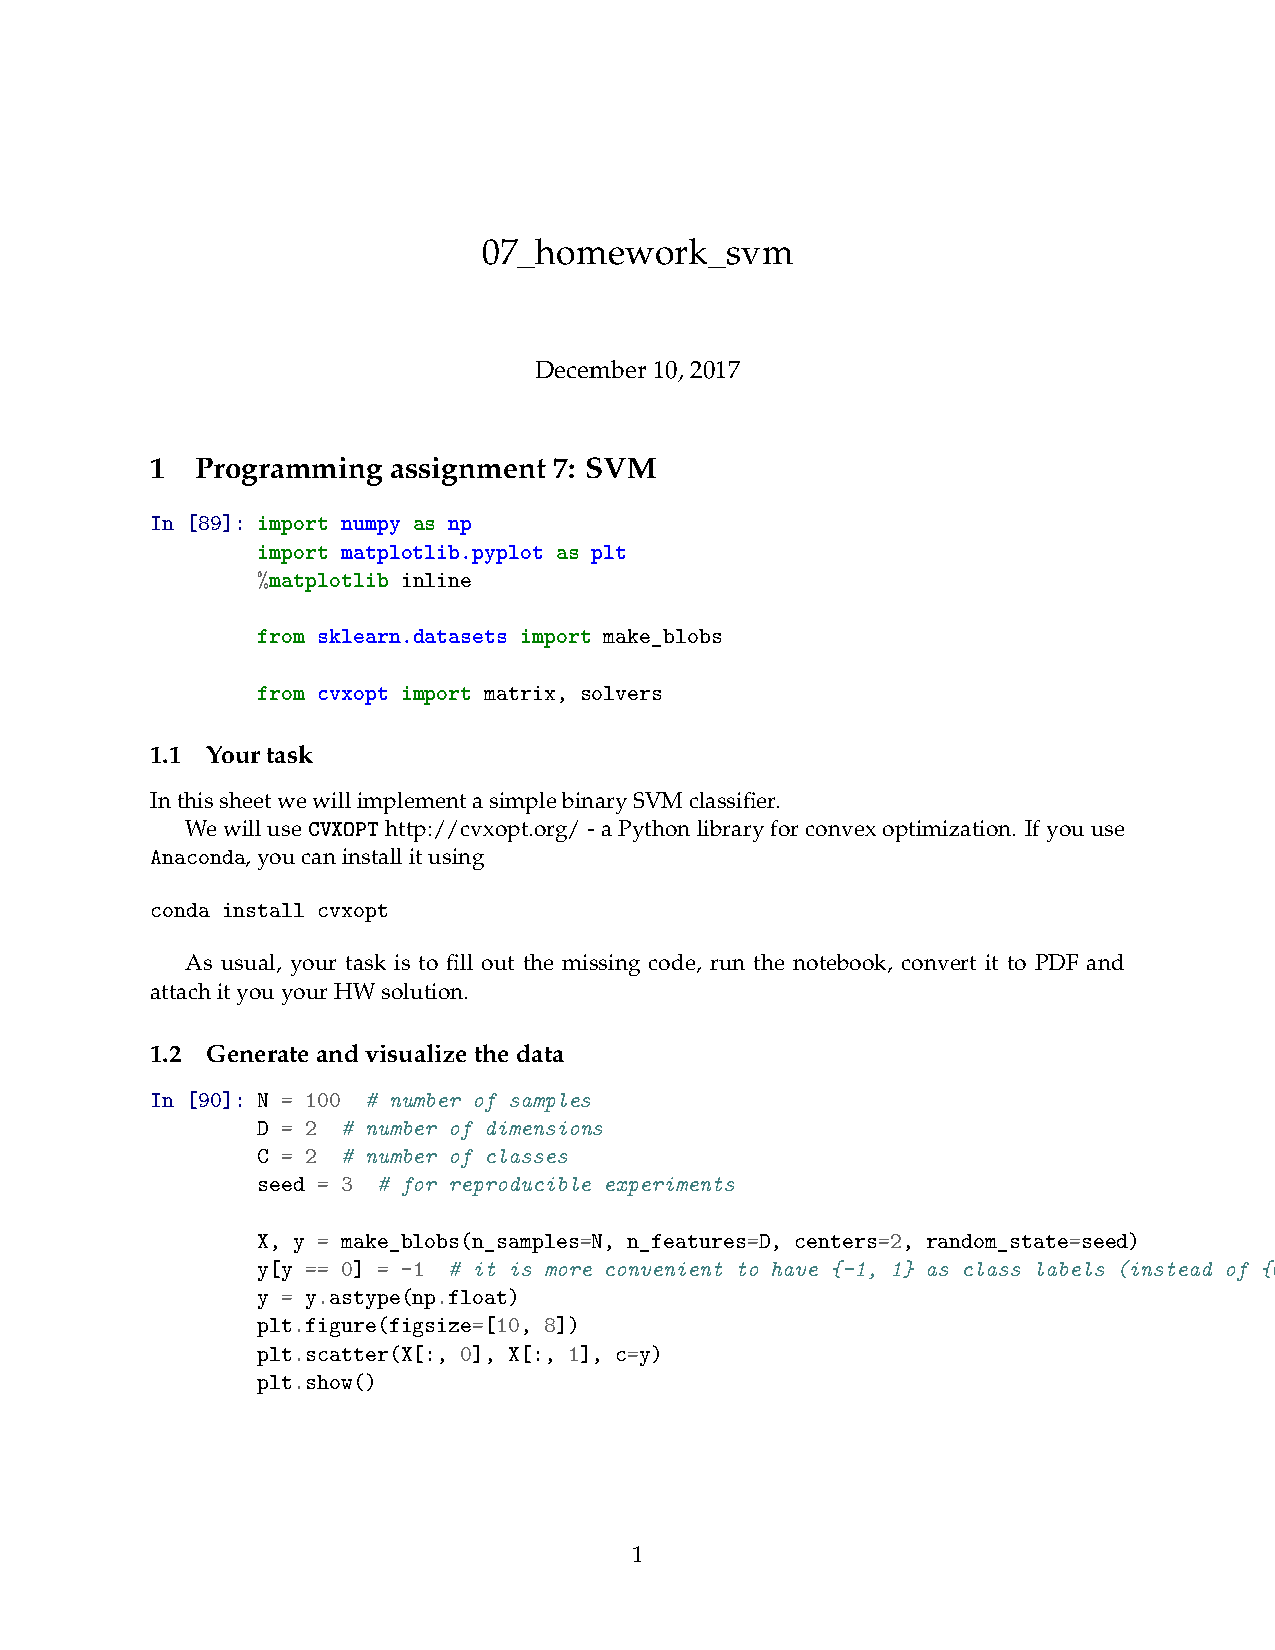
\includepdf[pages=-]{../07_homework_svm.pdf}
	
\end{document}
